\chapter{Preliminaries\label{chap:preliminaries}}

In this chapter, an overview of subjects that this work builds on is given.
The first section discusses propositional satisfiability, as this is the declarative paradigm the presented algorithm builds on.
Following that, bi-objective optimization is described, starting from a general perspective and ending up with notation used for bi-objective optimization in the context of propositional logic.
The chapter is concluded with a section overviewing different approaches to solving bi-objective optimization problems.
The focus hereby is on approaches based on propositional satisfiability, but others are briefly discussed as well.

\section{Propositional Satisfiability\label{sec:sat}}

For a Boolean variable $x$ there are two literals, the positive $x$ and the negative $\lnot x$. 
A clause $C$ is a set of (disjunction over) literals and a CNF formula $\formula$ is a set of (conjunction over) clauses.
A truth assignment $\sol$ maps boolean variables to $1$ (true) or $0$ (false).
The semantics of truth assignments are extended to a clause $C$ and a formula $\formula$ in the standard way: $\sol(C) = \max\{ \sol(l) \mid l \in C\}$ and $\sol(\formula) = \min\{\sol(C) \mid C \in \formula\}$.
When convenient, we view assignments $\sol$ over a set $X$ of variables as sets of literals $\sol = \{ x \mid x \in X,  \sol(x) = 1\} \cup \{ \lnot x \mid x \in X, \sol(x) = 0\}$.
An assignment $\sol$ for which $\sol(\formula) = 1$ is a solution to $\formula$.
The set of variables and literals appearing in $\formula$ are $\var(\formula)$ and $\lit(\formula)$, respectively.  
The propositional satisfiability (SAT) problem asks whether for a given formula $\formula$, a solution exists.
A formula $\formula$ is satisfiable if it has solutions, otherwise it is unsatisfiable.
\begin{example}
  Take the propositional formula $\formula_1 = a \land \lnot b$ over variables $\var(\formula_1) = \{a,b\}$.
  It is satisfiable since the assignment $\sol=(a,\lnot b)$ has $\sol(\formula_1)=1$.
  The formula $\formula_2 = a \land \lnot a$ on the other hand is not satisfiable since no assignment $\sol$ with $\sol(\formula_2)=1$ exists.
\end{example}

A SAT solver is an algorithm that solves the SAT problem for a given formula $\formula$.
If the formula is satisfiable, it returns ``satisfiable'' (SAT) and a solution $\sol$ with $\sol(\formula)=1$;
if it is unsatisfiable, it return ``unsatisfiable'' (UNSAT).

The SAT problem was proved $\mathcal{NP}$-complete in~\textcite{DBLP:conf/stoc/Cook71}.
This result is very central to its modern day use as a declarative programming approach to solving other $\mathcal{NP}$-complete problems by encoding them as a propositional formula first, solving them with a SAT solver and then decoding the solution to the original problem context.
The advantage of using SAT as a declarative programming language for solving other problems comes from the fact that---even though SAT is $\mathcal{NP}$-complete, and it is unclear if a polynomial time algorithm for solving it exists---conflict-driven clause learning solvers~\autocite{handbook2-cdcl} for SAT are efficient in practice and can solve problems with hundred-thousands of variables and clauses \TODO{check claim}.
\begin{example}
  Consider the problem of whether to wear tie and shirt to a given event with the following constraints:
  (i)~one should not wear a tie without a shirt, (ii)~not wearing a tie nor a shirt is impolite, and (iii)~wearing a shirt and a tie is considered overdressed.
  To solve this problem with the help of SAT, it can be encoded to propositional logic by introducing variables $v_\text{shirt}$ and $v_\text{tie}$ that represent if a shirt or a tie is worn.
  The constraint can then be encoded as the following clauses:
  $\clause_\text{(i)} = \lnot v_\text{tie} \lor v_\text{shirt}$, $\clause_\text{(ii)} = v_\text{tie} \lor v_\text{shirt}$ and $\clause_\text{(iii)} = \lnot v_\text{tie} \lor \lnot v_\text{shirt}$.
  The formula $\clause_\text{(i)} \land \clause_\text{(ii)} \land \clause_\text{(iii)}$ can then be solved with a SAT solver, which will return the satisfying assignment $\{ v_\text{shirt}, \lnot v_\text{tie} \}$.
  This solution is decoded as it being appropriate to wear a shirt but no tie.
  \TODO{can I use this example?}
\end{example}

In this work, w.l.o.g.\ we assume that all formulas are satisfiable \TODO{relevant?}.

\subsection{Incremental SAT Solving under Assumptions\label{sec:inc-sat}}

It is common that algorithms that solve problems with the help of SAT solvers produce a series of SAT problems that only differ slightly.
To be able to solve these subproblems more efficiently, most modern SAT solvers provide an incremental interface that allows for retaining information learned in previous solver calls \TODO{check if new CDCL chapter can be referenced}.
In order for the learned information from previous solver queries to still hold for subsequent calls, it is only possible to add clauses to the solvers internal formula, not remove them.
In addition, incremental SAT solvers support solving under assumptions.
The assumptions $\assump$ are a set of literals that are treated as unit clauses, i.e.\ a solver call with internal formula $\formula$ and assumptions $\assump$ either returns SAT and a solution $\sol \supset \assump$, or UNSAT and a subset $\core \subset \{\lnot l \mid l\in\assump\}$ such that $\formula \land \bigwedge_{l \in \core} (\lnot l)$ is unsatisfiable.
The subset $\core$ is called an unsatisfiable \emph{core} and, intuitively, is an explanation for the unsatisfiability of the query.

\subsection{Maximum Satisfiability\label{sec:max-sat}}

Maximum satisfiability (MaxSAT) is the optimization variant of the decision SAT problem.
In it, the goal is to find a solution that satisfies as many of the given clauses as possible.
Most commonly and in this work, MaxSAT refers to the extension of weighted partial MaxSAT, in which a set of \emph{hard} clauses $\formula$ and another set of \emph{soft} clauses $\softs$ are given.
Each clause $\clause \in \softs$ is assigned a weight $w_\clause$ and a solution $\sol$ that satisfies $\formula$ while minimizing $\sum_{\clause\in\softs \mid \tau(\clause)=0} w_\clause$ is optimal for the problem.

In the same way that SAT can be used as a declarative language to solve other decision problems, MaxSAT can be used to solve other optimization problems.

\subsection{Encoding Cardinality Constraints\label{sec:card-const}}

A common type of constraint to appear when encoding problems into SAT is that of a cardinality constraint.
Cardinality constraints, informally speaking, enforce a bound on how many literals in a set can be assigned to true.
Formally, for a set $L$ of literals and a bound $k \in \mathbb{N}$, $\texttt{As-CNF}\left(\sum_{l \in L} l \circ k\right)$ denotes a CNF formula that encodes the linear inequality $\sum_{l \in L} l \circ k$, where $\circ \in \{ ,< ,> ,\geq, \leq, =\}$.
Numerous methods of forming such CNF formulas are known~\autocite{DBLP:conf/cp/BailleuxB03}.
In this work we make use of the totalizer encoding.

Given a set $L$ of $n$ input literals and a bound $k=1, \ldots, n$, the (incremental) totalizer~\autocite{DBLP:conf/cp/BailleuxB03,DBLP:conf/cp/MartinsJML14} encoding produces a CNF formula $\tot(L, k)$ that defines a set $\{\ov{L}{1}, \ldots, \ov{L}{k}\} \subset \var(\tot(L))$ of \emph{output literals} that---informally speaking---count the number of literals in $L$ assigned to true by solutions to $\tot(L)$:
if $\tau$ is an assignment that satisfies $\tot(L)$, then $\tau(\ov{L}{b}) = 1$ if $\sum_{l \in L} \tau(l) < b$ \TODO{point out that iff (or $\leftarrow$) are possible as well, but we only need upper bounds)}.
The incremental totalizer supports both increasing the bound $k$ and adding new input literals without having to rebuild the whole formula:
we have that $\tot(L, k) \subset \tot(L, k')$ and $\tot(L, k) \subset  \tot(L \cup L', k)$ hold for any bound $k' > k$ and set $L'$ of literals for which $L \cap L' =  \emptyset$. 
We use $\ove{L}{k}$ as a shorthand for the literal $\ov{L}{k+1}$.
We note that the assignments of the auxiliary variables of the totalizer encoding are functionally defined by the assignment of the input and output variables.
As such we will leave them out from the solutions we describe in favour of brevity and clarity of examples. 

\section{Bi-Objective Optimization and Pareto Optimality\label{sec:biopt}}

Multi-objective optimization is the problem of optimizing $\nobj$ objective functions with the decision variable $x$, while $x$ has to be within the decision space $\feasible$.
W.l.o.g., we assume that all optimizations seek to minimize the objective function.
Formally a multi-objective optimization problem (MOOP) is the following:
\begin{equation}\label{eq:moop}
  \min (\generalobj_1(x),\generalobj_2(x),\dots,\generalobj_\nobj(x))\ \text{s.t.}\ x\in \feasible.
\end{equation}
For multi-objective optimization problems, since the objectives might be in conflict with each other, no single optimal solution exists.
However, the notions of domination and pareto optimality can be used.
\begin{definition}[Domination]
  Given a MOOP as defined in \cref{eq:moop} and two solutions $x,x' \in \feasible$, $x$ dominates $x'$ (w.r.t.\ $\generalobj_1,\dots,\generalobj_\nobj)$) is (i)~$\forall i\in\{1,\dots,\nobj\},\ \generalobj_i(x) \leq \generalobj_i(x')$, and (ii)~$\exists i\in\{1,\dots,\nobj\},\ \generalobj_i(x) < \generalobj_i(x')$.
  We represent $x$ dominating $x'$ as $x \prec x'$.
\end{definition}
\begin{definition}[Pareto optimality]
  Given a MOOP as defined in \cref{eq:moop}, a solution $x \in \feasible$ is pareto-optimal (w.r.t.\ $\generalobj_1,\dots,\generalobj_\nobj)$) iff $\nexists x' \in \feasible,\ x' \prec x$, i.e., it is not dominated by any other solution.
\end{definition}
When the objectives are clear from context, we will simply say that a solution $x$ is pareto-optimal.
Note that there can be multiple pareto-optimal solutions to a MOOP.
The set of all pareto-optimal solutions is called the pareto front (w.r.t.\ $\generalobj_1,\dots,\generalobj_\nobj)$); the tuple $(\generalobj_1(x),\dots,\generalobj_\nobj(x))$ for a pareto-optimal $x$ is a pareto point (which multiple solutions can correspond to).

The subset of all multi-objective optimization problems which this work provides a solving algorithm for, is \emph{bi}-objective optimization, where the number of objective functions $\nobj=2$.
Furthermore, we restrict the objective functions to be linear.
Bi-objective optimization problems can be solved by many approaches (see \cref{sec:approaches} for more details), but in this work we focus on SAT-based approaches.
We therefore formalize the problem in a context of propositional satisfiability.
An objective $\Obj$ is a multiset of literals, which allows for representing objective functions with non-unit coefficients.
The value $\Obj(\sol)$ of a truth assignment $\sol$ under $\Obj$ is $\Obj(\sol) = \sum_{l \in \Obj} \sol(l)$, i.e., the number of the literals in $\Obj$ that $\sol$ assigns to $1$. 
Weighted objectives are represented by adding a literal multiple times.
Formalizing the objectives this way and encoding the decision space $\feasible$ as a propositional formula $\formula$ is similar to MaxSAT, where $\formula$ resembles the hard clauses while the two objectives resemble two sets of (unit) soft clauses.
With our algorithm, we consider the task of computing a representative solution for each pareto point as well as the task of enumerating all solutions in the pareto front.

\begin{figure}
  \begin{minipage}{0.36\textwidth}
  \footnotesize
  \begin{align*}
  \formula = &\{ \texttt{As-CNF}\left(\sum_ {x \in \Obj_\inc \cup \Obj_\dec} x \geq 3 \right), \\
  			&(i_1 \lor i_2),  (i_2 \lor i_3), \\
		 &(d_1 \lor d_2), (d_2 \lor d_3) \} \\ \\
  \Obj_\dec =&\{ d_1,d_2, d_3\}   \\ 
  \Obj_\inc =&\{ i_1,i_2, i_3\}  
  \end{align*}
  \end{minipage}
  \;
  \begin{minipage}{0.6\textwidth}
    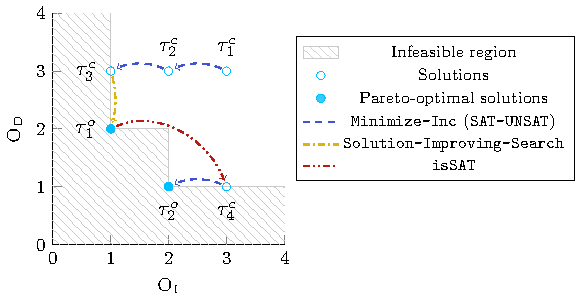
\includegraphics{search-trace.pdf}
  \end{minipage}
  \caption{Left: An example formula $\formula$ and two objectives $\Obj_\inc$ and $\Obj_\dec$.
    Right: the solution space of $\formula$ w.r.t.\ $\Obj_\inc$ and $\Obj_\dec$.
    The solutions $\tau^o_1$ and $\tau^o_2$ (solid points) are pareto-optimal, while $\tau^c_i$ for $i=1,\ldots,4$ are not.\label{fig:search-trace}}
\end{figure}

\begin{example}\label{ex:main}
  An example formula $\formula$ and two objectives $\Obj_\inc$ and $\Obj_\dec$ are shown on the left side of \cref{fig:search-trace}. 
  The solution space is illustrated on the right.
  The two solid dots correspond to the two pareto points of $\formula$ w.r.t.\ $\Obj_\inc$ and $\Obj_\dec$. 
  Examples of pareto-optimal solutions corresponding to these points are $\sol^o_1 = \{d_1, d_3, i_2, \lnot d_2, \lnot i_1, \lnot i_3\}$ and $\sol^o_2 = \{i_1, i_3, d_2, \lnot i_2, \lnot d_1, \lnot d_3\}$.
  The solution $\sol^c_3 = \{d_1, d_2, d_3, i_2, \lnot i_1, \lnot i_3\}$ is dominated by $\sol^o_1$ ($\sol^o_1 \prec \sol^c_e$) because $\Obj_\inc(\sol^o_1) \leq \Obj_\inc(\sol^c_3)$ and $\Obj_\dec(\sol^o_1) < \Obj_\dec(\sol^c_3)$.
\end{example}

An important property of pareto-optimal solutions to bi-objective problems is summarized by the next proposition.

\begin{proposition}[Adapted from~\autocite{DBLP:conf/aaai/HartertS14}] \label{prop:biobjective}
  Sorting the pareto-optimal solutions of $\formula$ w.r.t.\ increasing values of $\Obj_1$ is equivalent to sorting them w.r.t.\ decreasing values of $\Obj_2$ and vice-versa.
\end{proposition}

\begin{example}
  Consider the formula $\formula$, the objectives $\Obj_\inc$ and $\Obj_\dec$ and the two pareto-optimal solutions $\tau^o_1$ and $\tau^o_2$ from \cref{fig:search-trace} and \cref{ex:main}.
  By the definition of pareto-optimality, lowering the value of one objective of a pareto-optimal solution has to increase the value of the other;
  we have $\Obj_\inc(\tau^o_1) = 1 < 2 = \Obj_\inc(\tau^o_2)$ and $\Obj_\dec(\tau^o_1) = 2 > 1 = \Obj_\dec(\tau^o_2)$.
\end{example}

\section{Approaches to Bi-Objective Optimization\label{sec:approaches}}

\TODO{signposting}

\subsection{SAT-Based Approaches\label{sec:sat-based}}

\subsubsection{$P$-minimal Solution Enumeration\label{sec:p-minimal}}

The approach perhaps closest to ours is solving multi-objective constraint optimization problems by enumerating so-called $P$-minimal solutions~\autocite{DBLP:conf/cp/SohBTB17,DBLP:conf/ftp/KoshimuraNFH09}.
We were unable to obtain an implementation of the approach from the authors.
For a fair comparison with \algname{}, we hence reimplemented the approach similarly as \algname{}.
In more detail, the $P$-minimal approach  corresponds to enumerating the solutions of $\formula^\text{W} = \formula \land \tot(\Obj_{\inc}) \land \tot(\Obj_{\dec})$ that are subset-minimal w.r.t.\ the set of outputs of the totalizers.
More precisely, if $P$ is the set of output literals of $\tot(\Obj_{\inc}) \land \tot(\Obj_{\dec})$, then the goal is to enumerate solutions $\tau_m$ such that no other solution $\tau$ has $\{ b \mid b \in P \land \tau(b) = 0\} \subsetneq \{ b \mid b \in P \land \tau_m(b) = 0\}$.
The procedure for enumerating such solutions (detailed in~\textcite{DBLP:conf/ftp/KoshimuraNFH09}) works by (i)~using a solver to obtain any solution $\tau$ of $\formula^\text{W}$, (ii)~iteratively minimizing the subset of variables of $P$ set to true by the solution, and, once a minimal solution $\tau_m$ has been found, (iii)~adding the clause $(\ov{\Obj_{\inc}}{k_1} \lor \ov{\Obj_{\dec}}{k_2})$ containing the output variables corresponding to the lowest index set to true by $\tau_m$.

\begin{example}
  Consider the formula $\formula$ and two objectives $\Obj_\inc$ and $\Obj_\dec$ from \cref{fig:search-trace}.
  $P$-minimal starts by building two totalizers $\tot(\Obj_\inc)$ and $\tot(\Obj_\dec)$ and invoking the SAT solver on $\formula^\text{W} = \formula \land \tot(\Obj_\inc) \land \tot(\Obj_\dec)$.
  The result is satisfiable, assume the first solution obtained is $\tau^c_1 = \{i_1, i_2, i_3, d_1, d_2, d_3\}$. 
  In order to minimize $\tau^c_1$, the clause $(\ov{\Obj_\inc}{3} \lor \ov{\Obj_\dec}{3})$ is added to the SAT solver, and the solver is invoked again under the assumptions $\{ \ove{\Obj_\inc}{3}, \ove{\Obj_\dec}{3} \}$.
  The added clause blocks $\tau^c_1$ and all solutions dominated by $\tau^c_1$ from the search space.
  Assume the next solution obtained is $\tau^c_5 = \{d_1, d_3, i_1, i_3, \lnot d_2, \lnot i_2\}$. 
  Again, a clause $(\ov{\Obj_\inc}{2} \lor \ov{\Obj_\dec}{2})$ is added, and the SAT solver is queried with assumptions $\{ \ove{\Obj_\inc}{2}, \ove{\Obj_\dec}{2} \}$.
  The result is SAT, assume the solution obtained is $\tau^o_2 = \{ i_1, i_3, d_2, \lnot i_2, \lnot d_2, \lnot d_3\}$. 
  $P$-minimal then adds the clause $(\ov{\Obj_\inc}{2} \lor \ov{\Obj_\dec}{1})$ and invokes the solver again under the assumptions $\{ \ove{\Obj_\inc}{2}, \ove{\Obj_\dec}{1} \}$.
  The result is UNSAT which proves that $\tau^o_2$ is pareto-optimal. 
  To find a next pareto-optimal solution, the solver is queried without any assumptions for a new solution to start the minimization process from.
\end{example}

Note that $P$-minimal has no guarantee on the order that the solutions are enumerated in. 
Intuitively, when an intermediate solution $\tau$ is found, the following SAT solver call either provides another solution that dominates $\tau$, or proves that $\tau$ is pareto-optimal.  

%As presented in~\cite{DBLP:conf/cp/SohBTB17}, $P$-minimal will only enumerate a single solution per pareto point.
In our implementation we extended $P$-minimal to the task of enumerating all solutions on the pareto front.
Specifically, we add a new relaxation variable $r$ to the clause added each iteration for use as an assumption to enumerate all solutions at that pareto point in a standard way.
If the next solution found dominates the previous one, we harden the clause added at the previous iteration by adding $\lnot r$ as a unit clause.
Also, once all solutions for that pareto point are enumerated, the clause is hardened.

\subsubsection{Enumeration of Pareto-Minimal Correction Sets\label{sec:pareto-mcs}}

In~\textcite{DBLP:conf/ijcai/Terra-NevesLM18a,DBLP:conf/aaai/Terra-NevesLM18,DBLP:conf/ijcai/Terra-NevesLM18} an approach for computing pareto-optimal solutions via so-called pareto-minimal correction sets (paretoMCSes) was proposed.
%A paretoMCS  consists  of two sets of literals $(M_1, M_2)$  such that  (i)~$M_1 \subset \Obj_1$ and $M_2 \subset \Obj_2$, and (ii)~there is
%a pareto-optimal solution $\tau$ that sets $\tau(o) = 1$ for all $o \in M_1 \cup M_2$ and $\tau(o) = 0$ for all other $o \in (\Obj_1 \cup \Obj_2) \setminus (M_1 \cup M_2)$.
%In~\cite{DBLP:conf/ijcai/Terra-NevesLM18a}, the computation of pareto-optimal solutions is reduced into the computation of paretoMCSes.
%The  task computing paretoMCSes is  accomplished in~\cite{DBLP:conf/ijcai/Terra-NevesLM18a}
In terms of our notation, the approach works by enumerating all subsets $S \subset  (\Obj_{\inc} \cup \Obj_{\dec})$ for which (i) $\formula \land \bigwedge_{l \in  (\Obj_{\inc} \cup \Obj_\dec) \setminus S} (\lnot l)$ is satisfiable and (ii) $\formula \land \bigwedge_{l \in  (\Obj_{\inc} \cup \Obj_\dec) \setminus S'} (\lnot l)$ is unsatisfiable for all $S' \subsetneq S$.
%(i)~there is a \emph{corresponding solution} $\tau^S$ that sets $\tau^S(o) = 1$ for all $o \in S$ and $\tau(S) = 0$ for all $o \in  (\Obj_1 \cup \Obj_2) \setminus S$, and (ii)~no such solution exists for any $S' \subsetneq S$.
Let $\mathcal{S}$ be the collection of all such sets.
The computation of $\mathcal{S}$ corresponds to MCS enumeration to which numerous algorithms have been proposed~\autocite{DBLP:conf/lpar/BendikC20,DBLP:conf/hvc/MorgadoLM12,DBLP:conf/sat/PrevitiMJM17}.
The pareto-optimal solutions are obtained by extracting the solutions satisfying $\formula \land \bigwedge_{l \in  (\Obj_{\inc} \cup \Obj_\dec) \setminus S} (\lnot l)$ for all $S \in \mathcal{S}$ and removing the dominated ones~\cite{DBLP:conf/ijcai/Terra-NevesLM18a}.
The paretoMCS approach to multi-objective optimization is approximative in that it can only guarantee that a solution is pareto-optimal once the full set $\mathcal{S}$ has been computed.
In contrast, every minimal solution found during the $P$-minimal approach of~\textcite{DBLP:conf/cp/SohBTB17} and every solution returned by the $\E$ subroutine of \cref{alg:base-algorithm} is immediately known to be pareto-optimal.
\begin{example}\label{ex:MCS}
  Consider the formula $\formula$ and two objectives $\Obj_\inc$ and $\Obj_\dec$ from \cref{fig:search-trace}.
  The paretoMCS enumeration procedure will return the solution $\tau = \{d_1, d_3, i_1, i_3\}$ since no solution $\tau_s$ of $\formula$ has $\{x \in \Obj_\inc \cup \Obj_\dec \mid  \tau_s(x) = 1\} \subsetneq \{d_1, d_3, i_1, i_3\}$.
  The solution $\tau$ is not pareto-optimal, but only filtered out in the end when all solutions in $\mathcal{S}$ have been enumerated.
\end{example}
The fact that the solution $\tau$ is not pareto-optimal can only be discovered when a solution that dominates it is enumerated. 
However, there are no guarantees on when such a dominating solution is found. 

\subsubsection{Implicit Hitting Set: Seesaw\label{sec:seesaw}}

Seesaw~\autocite{DBLP:conf/cp/JanotaMSM21} was recently proposed as a framework for bi-objective optimization as a generalization of the so-called implicit hitting set approach~\autocite{DBLP:conf/cp/DaviesB13,DBLP:conf/cp/IgnatievPLM15,DBLP:conf/kr/SaikkoWJ16,DBLP:conf/cade/FazekasBB18,DBLP:conf/kr/SaikkoDAJ18}.
In contrast to our work, a main ingredient in Seesaw is the idea of treating one of the objectives as a black box.
This allows for---but also requires---problem-specific instantiations of the black box;
no generic Seesaw implementation applicable generally to bi-objective optimization is available.
That said, to enable a comparison with (an instantiation of) Seesaw, we instantiated the approach for the LIDR problem.
(For bi-objective set covering, both objectives are monotone over the chosen cover;
instantiating Seesaw is not feasible because the refined core extraction method from~\textcite{DBLP:conf/cp/JanotaMSM21} cannot be used, resulting in enumerating all possible solutions.)

While the original paper presents Seesaw in general terms, in our context the Seesaw algorithm computes pareto-optimal solutions of a formula $\formula$ by maintaining a collection $\cores$ of subsets of $\Obj_\inc$ that are called \emph{cores}.
Informally speaking, every solution $\tau$ that improves on $\Obj_\dec$ needs to assign at least one literal from each core to $1$.
The algorithm works iteratively by computing a hitting set $\hs \subset \Obj_\inc$ (using an integer programming solver, in our case CPLEX 20.10), i.e., a subset-minimal set of literals of $\Obj_\inc$ that intersects with each core in $\mathcal{C}$, and then a solution $\tau$ that sets $\tau(o) = 1$ for each $o \in \hs$ and $\tau(o) = 0$ for each $o \in \Obj_\inc \setminus \hs$ and for which $\Obj_\dec(\tau)$ is the smallest possible value for all such solutions if one exists.
The iteration then extracts a new core that $\hs$ does not intersect with.
The pareto-optimal solutions of $\formula$ are identified by the size of the hitting set increasing.
More precisely, if the hitting set is found to increase from size $|\hs|$ to size $|\hs_2|$ with $|\hs_2|>|\hs|$, the solution $\tau$ found with a hitting set of size $|\hs|$ that has the smallest minimal value $\Obj_\dec(\tau)$ is pareto-optimal~\autocite{DBLP:conf/cp/JanotaMSM21}.

We instantiated Seesaw for LIDR by using misclassifications as the objective over which cores are extracted and a hitting set $\hs$ is found with the help of CPLEX over these cores.
In the second step, the number of literals in the smallest rule misclassifying the examples in $\hs$ or a subset of it is found.
This function is implemented as a solution-improving search  in CaDiCaL.
This instantiation was chosen because finding the smallest rule misclassifying $\hs$ is an anti-monotone function and the refined version of core extraction presented in~\textcite{DBLP:conf/cp/JanotaMSM21} can therefore be used, making Seesaw feasible in the first place.

\begin{example}
  Consider the formula $\formula$ and two objectives $\Obj_\inc$ and $\Obj_\dec$ from \cref{fig:search-trace}. 
  Initially there are no cores, so $\cores = \emptyset$. As such the first hitting set $\hs = \emptyset$ will also be empty.
  Since there are no solutions $\tau$ that set $\tau(u) = 0$ for each $u \in \Obj_\inc$, the iteration ends by extracting $\Obj_\inc$ as a core. 
  The intuition here is that at this point, we know that any solution $\tau$ of $\formula$ sets at least one variable in $\Obj_\inc$ to $1$.

  In the next iteration, a hitting set over $\cores = \{ \Obj_\inc \}$ is computed. There are a number of alternatives for such hitting sets, assume $\hs = \{ i_1 \}$.
  Since there are no solutions $\tau$ of $\formula$ that set $\tau(i_2) = \tau(i_3) = 0$, the iteration ends with extracting $\{ i_2, i_3\}$ as a new core.
  At this point we know that any solution sets at least one variable of $\Obj_\inc$ and one from $\{i_2, i_3\}$ to $1$.

  Assume the next hitting set computed is $\hs = \{i_2\}$. Now there actually are solutions $\tau$ of $\formula$ that set $\tau(i_1) = \tau(i_3) = 0$, one that minimizes 
  $\Obj_\dec(\tau)$ is $\tau^o_1 = \{d_1, d_3, i_2, \lnot d_2, \lnot i_1, \lnot i_3 \}$. The iteration ends with extracting the core
  $\kappa = \{i_1, i_3\}$. Now the intuition is that, since $\tau^o_1$ minimizes $\Obj_\dec$ over solutions that assign $\tau(u) = 0$ for every $u \notin \hs$, every solution that obtains a lower value of $\Obj_\dec$
  assigns at least one literal of $\kappa$ to $1$ as well. 

  In the next iteration, the set $\cores$ of cores is $\cores = \{ \Obj_\inc, \{i_2, i_3\}, \{i_1, i_3\}\}$. The only subset minimal hitting set $\hs$ of $\cores$ is $\hs = \{i_3\}$.
  There are no solutions $\tau$ that set $\tau(i_1) = \tau(i_2) = 0$ so a new core $\{i_1, i_2\}$ is extracted. 
  In the next iteration, one possible hitting set is $\hs = \{i_1, i_3\}$. Since the size of the hitting set grew from $1$ to $2$, the algorithm concludes that $\tau^o_1$ is pareto-optimal. 
  In this iteration, the pareto-optimal solution $\tau^o_2 = \{d_2, i_1, i_3, \lnot d_1, \lnot d_3, \lnot i_2 \}$ is obtained 
  as the solution that minimizes $\Obj_\dec$ over all solutions $\tau$ that set $\tau(i_2) = 0$.  

  The algorithm continues in this manner, computing the hitting sets, $\{i_1, i_2\}$, $\{i_2, i_3\}$ and $\{i_1, i_2, i_3\}$. 
  After computing the hitting set consisting of all literals in $\Obj_\inc$, the core extracted is $\emptyset$ at which point the algorithm terminates. 
\end{example}

%Note that the core-extraction strategy that only computes $\Obj_\inc \setminus \hs$ as the new core detailed in the example corresponds to what is called the weakest possible strategy in~\cite{DBLP:conf/cp/JanotaMSM21}.
%For the comparison
%we implemented also
%the improvements to SeeSaw proposed in~\cite{DBLP:conf/cp/JanotaMSM21} as the original authors  mention that the weakest strategy essentially reduces to enumerating
%all subsets of $\Obj_\inc$, thus being infeasible in practice. 
Note that, in contrast to $\algname$ and $P$-minimal, extending Seesaw as it is presented in~\textcite{DBLP:conf/cp/JanotaMSM21} to support the enumeration of all pareto-optimal solutions seems non-trivial.
For a non-formal intuition note that, while Seesaw is guaranteed to find at least one solution obtaining the objective values of each pareto-optimal point, the non-deterministic hitting set computation might steer the algorithm past other solutions that obtain the same values.

\subsubsection{SAT-Based Lexicographic Optimization\label{sec:lex-opt}}

\subsection{Other Declarative Optimization Paradigms\label{sec:other-approaches}}

\subsection{Approximative Approaches\label{sec:approximative}}
